\documentclass[tikz, border=5pt]{standalone}

\usepackage[utf8]{inputenc}
\usepackage[T1]{fontenc}
\usepackage{cmap}
\usepackage{amsmath}
\usepackage{amssymb}
\usepackage{verbatim}
\usepackage{bm}
\usepackage{siunitx}

\renewcommand{\familydefault}{\sfdefault}
\usepackage[cm]{sfmath}

\usepackage{tikz}
\usetikzlibrary{math}
\usetikzlibrary{bending}
\usetikzlibrary{decorations.pathreplacing}
\usetikzlibrary{decorations.pathmorphing}
\usetikzlibrary{fadings}
\usetikzlibrary{positioning}
\definecolor{cblue}{rgb}{0.396, 0.643, 0.82}
\definecolor{corange}{rgb}{1.0, 0.69, 0.416}
\definecolor{cgreen}{rgb}{0.471, 0.824, 0.471}
\definecolor{cred}{rgb}{1.0, 0.502, 0.502}
\definecolor{cpurple}{rgb}{0.863, 0.78, 0.937}

\begin{document}
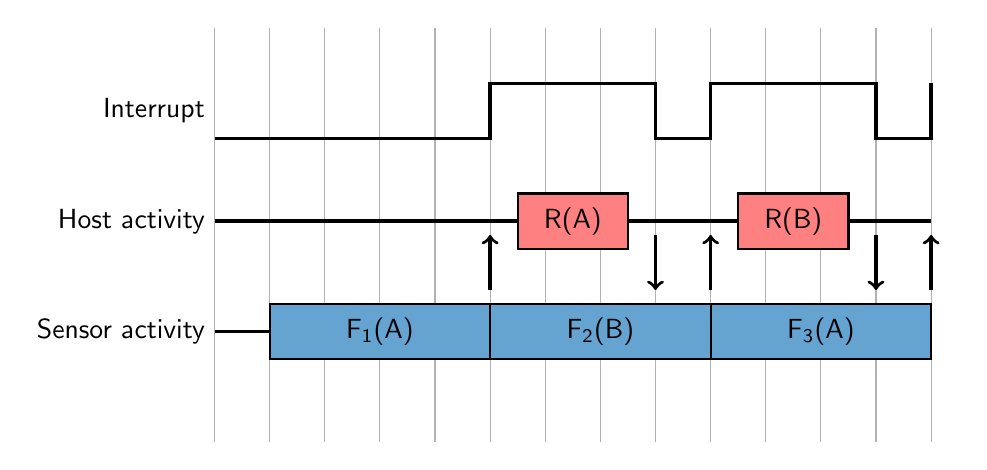
\begin{tikzpicture}[scale=0.7]
  \draw [thin, black!30, ystep=0] (0, -2) grid (13.5, 5.5);

  \node at (0, 0) [left] {Sensor activity};
  \draw [very thick] (0, 0) -- ++(13, 0);

  \draw [fill=cblue, thick] (1, -0.5) rectangle ++(4, 1) node[midway] {$\text{F}_1(\text{A})$};
  \draw [fill=cblue, thick] (5, -0.5) rectangle ++(4, 1) node[midway] {$\text{F}_2(\text{B})$};
  \draw [fill=cblue, thick] (9, -0.5) rectangle ++(4, 1) node[midway] {$\text{F}_3(\text{A})$};

  \draw [very thick, ->] (5, 0.75) -- ++(0, 1);
  \draw [very thick, <-] (8, 0.75) -- ++(0, 1);
  \draw [very thick, ->] (9, 0.75) -- ++(0, 1);
  \draw [very thick, <-] (12, 0.75) -- ++(0, 1);
  \draw [very thick, ->] (13, 0.75) -- ++(0, 1);

  \node at (0, 2) [left] {Host activity};
  \draw [very thick] (0, 2) -- ++(13, 0);
  \draw [fill=cred, thick] (5.5, 1.5) rectangle ++(2, 1) node[midway] {R(A)};
  \draw [fill=cred, thick] (9.5, 1.5) rectangle ++(2, 1) node[midway] {R(B)};

  \node at (0, 4) [left] {Interrupt};
  \draw [very thick] (0, 3.5)
    -- ++(1, 0)
    -- ++(4, 0)
    -- ++(0, 1)
    -- ++(3, 0)
    -- ++(0, -1)
    -- ++(1, 0)
    -- ++(0, 1)
    -- ++(3, 0)
    -- ++(0, -1)
    -- ++(1, 0)
    -- ++(0, 1)
    ;
\end{tikzpicture}
\end{document}
